% Options for packages loaded elsewhere
\PassOptionsToPackage{unicode}{hyperref}
\PassOptionsToPackage{hyphens}{url}
%
\documentclass[
  ignorenonframetext,
]{beamer}
\usepackage{pgfpages}
\setbeamertemplate{caption}[numbered]
\setbeamertemplate{caption label separator}{: }
\setbeamercolor{caption name}{fg=normal text.fg}
\beamertemplatenavigationsymbolsempty
% Prevent slide breaks in the middle of a paragraph
\widowpenalties 1 10000
\raggedbottom
\setbeamertemplate{part page}{
  \centering
  \begin{beamercolorbox}[sep=16pt,center]{part title}
    \usebeamerfont{part title}\insertpart\par
  \end{beamercolorbox}
}
\setbeamertemplate{section page}{
  \centering
  \begin{beamercolorbox}[sep=12pt,center]{part title}
    \usebeamerfont{section title}\insertsection\par
  \end{beamercolorbox}
}
\setbeamertemplate{subsection page}{
  \centering
  \begin{beamercolorbox}[sep=8pt,center]{part title}
    \usebeamerfont{subsection title}\insertsubsection\par
  \end{beamercolorbox}
}
\AtBeginPart{
  \frame{\partpage}
}
\AtBeginSection{
  \ifbibliography
  \else
    \frame{\sectionpage}
  \fi
}
\AtBeginSubsection{
  \frame{\subsectionpage}
}
\usepackage{amsmath,amssymb}
\usepackage{lmodern}
\usepackage{iftex}
\ifPDFTeX
  \usepackage[T1]{fontenc}
  \usepackage[utf8]{inputenc}
  \usepackage{textcomp} % provide euro and other symbols
\else % if luatex or xetex
  \usepackage{unicode-math}
  \defaultfontfeatures{Scale=MatchLowercase}
  \defaultfontfeatures[\rmfamily]{Ligatures=TeX,Scale=1}
\fi
% Use upquote if available, for straight quotes in verbatim environments
\IfFileExists{upquote.sty}{\usepackage{upquote}}{}
\IfFileExists{microtype.sty}{% use microtype if available
  \usepackage[]{microtype}
  \UseMicrotypeSet[protrusion]{basicmath} % disable protrusion for tt fonts
}{}
\makeatletter
\@ifundefined{KOMAClassName}{% if non-KOMA class
  \IfFileExists{parskip.sty}{%
    \usepackage{parskip}
  }{% else
    \setlength{\parindent}{0pt}
    \setlength{\parskip}{6pt plus 2pt minus 1pt}}
}{% if KOMA class
  \KOMAoptions{parskip=half}}
\makeatother
\usepackage{xcolor}
\newif\ifbibliography
\usepackage{color}
\usepackage{fancyvrb}
\newcommand{\VerbBar}{|}
\newcommand{\VERB}{\Verb[commandchars=\\\{\}]}
\DefineVerbatimEnvironment{Highlighting}{Verbatim}{commandchars=\\\{\}}
% Add ',fontsize=\small' for more characters per line
\usepackage{framed}
\definecolor{shadecolor}{RGB}{248,248,248}
\newenvironment{Shaded}{\begin{snugshade}}{\end{snugshade}}
\newcommand{\AlertTok}[1]{\textcolor[rgb]{0.94,0.16,0.16}{#1}}
\newcommand{\AnnotationTok}[1]{\textcolor[rgb]{0.56,0.35,0.01}{\textbf{\textit{#1}}}}
\newcommand{\AttributeTok}[1]{\textcolor[rgb]{0.77,0.63,0.00}{#1}}
\newcommand{\BaseNTok}[1]{\textcolor[rgb]{0.00,0.00,0.81}{#1}}
\newcommand{\BuiltInTok}[1]{#1}
\newcommand{\CharTok}[1]{\textcolor[rgb]{0.31,0.60,0.02}{#1}}
\newcommand{\CommentTok}[1]{\textcolor[rgb]{0.56,0.35,0.01}{\textit{#1}}}
\newcommand{\CommentVarTok}[1]{\textcolor[rgb]{0.56,0.35,0.01}{\textbf{\textit{#1}}}}
\newcommand{\ConstantTok}[1]{\textcolor[rgb]{0.00,0.00,0.00}{#1}}
\newcommand{\ControlFlowTok}[1]{\textcolor[rgb]{0.13,0.29,0.53}{\textbf{#1}}}
\newcommand{\DataTypeTok}[1]{\textcolor[rgb]{0.13,0.29,0.53}{#1}}
\newcommand{\DecValTok}[1]{\textcolor[rgb]{0.00,0.00,0.81}{#1}}
\newcommand{\DocumentationTok}[1]{\textcolor[rgb]{0.56,0.35,0.01}{\textbf{\textit{#1}}}}
\newcommand{\ErrorTok}[1]{\textcolor[rgb]{0.64,0.00,0.00}{\textbf{#1}}}
\newcommand{\ExtensionTok}[1]{#1}
\newcommand{\FloatTok}[1]{\textcolor[rgb]{0.00,0.00,0.81}{#1}}
\newcommand{\FunctionTok}[1]{\textcolor[rgb]{0.00,0.00,0.00}{#1}}
\newcommand{\ImportTok}[1]{#1}
\newcommand{\InformationTok}[1]{\textcolor[rgb]{0.56,0.35,0.01}{\textbf{\textit{#1}}}}
\newcommand{\KeywordTok}[1]{\textcolor[rgb]{0.13,0.29,0.53}{\textbf{#1}}}
\newcommand{\NormalTok}[1]{#1}
\newcommand{\OperatorTok}[1]{\textcolor[rgb]{0.81,0.36,0.00}{\textbf{#1}}}
\newcommand{\OtherTok}[1]{\textcolor[rgb]{0.56,0.35,0.01}{#1}}
\newcommand{\PreprocessorTok}[1]{\textcolor[rgb]{0.56,0.35,0.01}{\textit{#1}}}
\newcommand{\RegionMarkerTok}[1]{#1}
\newcommand{\SpecialCharTok}[1]{\textcolor[rgb]{0.00,0.00,0.00}{#1}}
\newcommand{\SpecialStringTok}[1]{\textcolor[rgb]{0.31,0.60,0.02}{#1}}
\newcommand{\StringTok}[1]{\textcolor[rgb]{0.31,0.60,0.02}{#1}}
\newcommand{\VariableTok}[1]{\textcolor[rgb]{0.00,0.00,0.00}{#1}}
\newcommand{\VerbatimStringTok}[1]{\textcolor[rgb]{0.31,0.60,0.02}{#1}}
\newcommand{\WarningTok}[1]{\textcolor[rgb]{0.56,0.35,0.01}{\textbf{\textit{#1}}}}
\usepackage{longtable,booktabs,array}
\usepackage{calc} % for calculating minipage widths
\usepackage{caption}
% Make caption package work with longtable
\makeatletter
\def\fnum@table{\tablename~\thetable}
\makeatother
\usepackage{graphicx}
\makeatletter
\def\maxwidth{\ifdim\Gin@nat@width>\linewidth\linewidth\else\Gin@nat@width\fi}
\def\maxheight{\ifdim\Gin@nat@height>\textheight\textheight\else\Gin@nat@height\fi}
\makeatother
% Scale images if necessary, so that they will not overflow the page
% margins by default, and it is still possible to overwrite the defaults
% using explicit options in \includegraphics[width, height, ...]{}
\setkeys{Gin}{width=\maxwidth,height=\maxheight,keepaspectratio}
% Set default figure placement to htbp
\makeatletter
\def\fps@figure{htbp}
\makeatother
\setlength{\emergencystretch}{3em} % prevent overfull lines
\providecommand{\tightlist}{%
  \setlength{\itemsep}{0pt}\setlength{\parskip}{0pt}}
\setcounter{secnumdepth}{-\maxdimen} % remove section numbering
\ifLuaTeX
  \usepackage{selnolig}  % disable illegal ligatures
\fi
\IfFileExists{bookmark.sty}{\usepackage{bookmark}}{\usepackage{hyperref}}
\IfFileExists{xurl.sty}{\usepackage{xurl}}{} % add URL line breaks if available
\urlstyle{same} % disable monospaced font for URLs
\hypersetup{
  hidelinks,
  pdfcreator={LaTeX via pandoc}}

\author{}
\date{\vspace{-2.5em}}

\begin{document}

\begin{frame}
\begin{longtable}[]{@{}l@{}}
\toprule()
\endhead
tle: `Session3: Visualisation avec ggplot' \\
thor: ``Visseho Adjiwanou, PhD.'' \\
stitute: ``SICSS - Montréal'' \\
te: ``14 June 2023'' \\
tput: \\
slidy\_presentation: default \\
beamer\_presentation: \\
colortheme: beaver \\
fonttheme: structurebold \\
theme: Antibes \\
ioslides\_presentation: default \\
ader-includes: \\
- \\
\bottomrule()
\end{longtable}
\end{frame}

\begin{frame}{Remerciements}
\protect\hypertarget{remerciements}{}
Robert Djogbénou, Georges Tchango et Nima Zahedinameghi ont contribué à
développer les cours de cette école d'été.
\end{frame}

\begin{frame}{Plan}
\protect\hypertarget{plan}{}
\begin{itemize}
\tightlist
\item
  Introduction
\item
  Type de graphiques pour les distributions univariées et bivariées
\item
  Présentation de ggplot de tidyverse
\item
  Visualisation de distribution univariée
\item
  Visualisation de distribution bivariée
\item
  Remarques
\item
  Ressources
\end{itemize}
\end{frame}

\hypertarget{introduction}{%
\section{Introduction}\label{introduction}}

\begin{frame}[fragile]{Introduction}
\protect\hypertarget{introduction-1}{}
\begin{itemize}
\item
  R dispose de plusieurs systèmes pour créer des graphiques, mais
  ggplot2 est l'un des plus élégants et des plus polyvalents.
\item
  Avec ggplot2, vous pouvez faire plus rapidement en apprenant un
  système et en l'appliquant à de nombreux graphiques.
\item
  Parce qu'il fait partie de \texttt{tidyverse}:
\item
  Il sera chargé automatiquement une fois que vous chargez tidyverse;
\item
  Il va fonctionner sur les bases de données ou les \texttt{tribbles}
\end{itemize}
\end{frame}

\begin{frame}[fragile]{Introduction}
\protect\hypertarget{introduction-2}{}
\begin{Shaded}
\begin{Highlighting}[]
\FunctionTok{library}\NormalTok{(tidyverse)}
\end{Highlighting}
\end{Shaded}

\begin{verbatim}
## -- Attaching core tidyverse packages ------------------------ tidyverse 2.0.0 --
## v dplyr     1.1.2     v readr     2.1.4
## v forcats   1.0.0     v stringr   1.5.0
## v ggplot2   3.4.1     v tibble    3.2.1
## v lubridate 1.9.2     v tidyr     1.3.0
## v purrr     1.0.1     
## -- Conflicts ------------------------------------------ tidyverse_conflicts() --
## x dplyr::filter() masks stats::filter()
## x dplyr::lag()    masks stats::lag()
## i Use the conflicted package (<http://conflicted.r-lib.org/>) to force all conflicts to become errors
\end{verbatim}
\end{frame}

\begin{frame}{Introduction}
\protect\hypertarget{introduction-3}{}
\begin{itemize}
\item
  Les graphiques nous permettent de répondre à plusieurs types de
  questions :
\item
  Quelle est la distribution d'une variable?
\item
  Est-ce que les filles ont plus tendances à vivre dans un type
  particulier de structure familiale?
\item
  Comment est-ce que la structure de la famille affecte la santé des
  enfants?
\item
  Est-ce qu'il existe une association entre les attitudes envers la
  violence conjugale et le niveau de scolarisation (données dhs\_ipv)
\item
  Cette relation est-elle positive? négative? ou nulle?
\end{itemize}
\end{frame}

\hypertarget{type-de-graphiques-pour-les-distributions-univariuxe9es-et-bivariuxe9es}{%
\section{Type de graphiques pour les distributions univariées et
bivariées}\label{type-de-graphiques-pour-les-distributions-univariuxe9es-et-bivariuxe9es}}

\begin{frame}{Les types de graphiques}
\protect\hypertarget{les-types-de-graphiques}{}
\begin{itemize}
\item
  Dépendent en général du type de variable (qualitative ou quantitative)
  et du nombre de variables
\item
  Graphiques pour representer une seule variable:
\end{itemize}

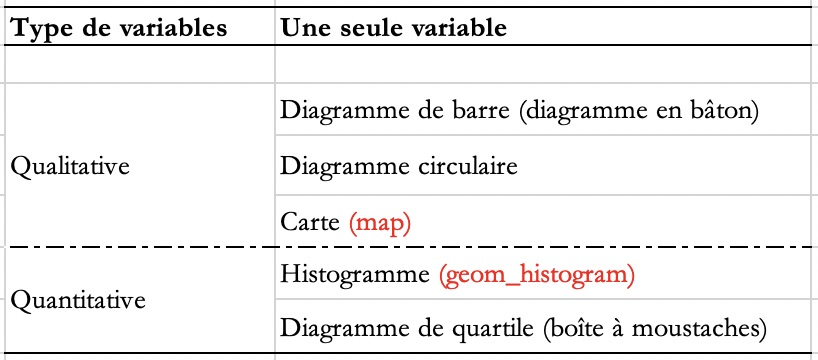
\includegraphics{../données/graphique1.jpg}
\end{frame}

\begin{frame}{Les types de graphiques}
\protect\hypertarget{les-types-de-graphiques-1}{}
\begin{itemize}
\tightlist
\item
  Graphiques pour representer l'association entre deux variables
\end{itemize}

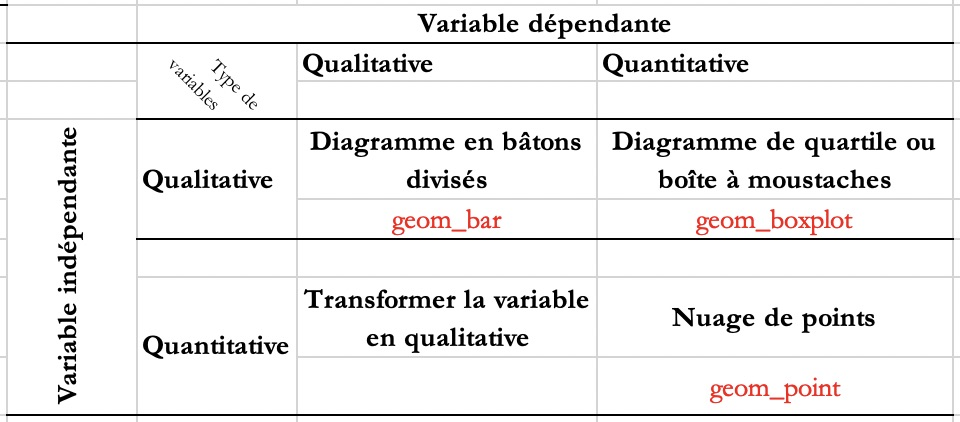
\includegraphics{../données/graphique2.jpg}
\end{frame}

\hypertarget{ggplot}{%
\section{ggplot}\label{ggplot}}

\begin{frame}{Forme générale}
\protect\hypertarget{forme-guxe9nuxe9rale}{}
\begin{itemize}
\tightlist
\item
  La forme générale d'un code de graphique est la suivante:
\end{itemize}

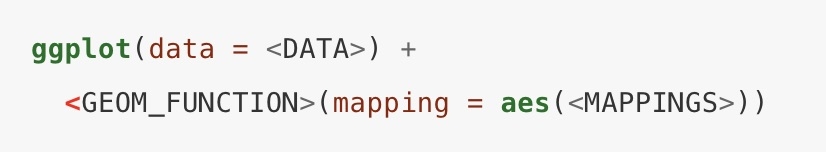
\includegraphics{../données/ggplot_forme_generale.jpg}

\begin{enumerate}
\tightlist
\item
  \textbf{ggplot} spécifie que vous utilisez la commande ggplot. C'est à
  ce niveau que vous spécifiez les données que vous voulez utiliser.
\end{enumerate}

\begin{itemize}
\tightlist
\item
  Ce n'est pas toujours obligatoire si vous utilisez plus d'une base de
  données.
\end{itemize}
\end{frame}

\begin{frame}{Forme générale}
\protect\hypertarget{forme-guxe9nuxe9rale-1}{}
\begin{itemize}
\tightlist
\item
  La forme générale d'un code de graphique est le suivant:
\end{itemize}

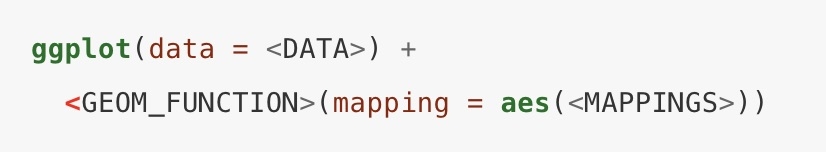
\includegraphics{../données/ggplot_forme_generale.jpg}

\begin{enumerate}
\setcounter{enumi}{1}
\tightlist
\item
  \textbf{geom\_function}, contient plusieurs fonctions pour spécifier
  le type de graphique que vous voulez faire. Le type de graphique
  indique le nombre de paramètres à inclure.
\end{enumerate}

\begin{itemize}
\tightlist
\item
  Exemples: geom\_histogram() pour les \textbf{histogrammes}
\item
  geom\_point() pour les \textbf{diagrammes de dispertions},
\item
  geom\_barplot() pour les \textbf{diagrammes de barre}.
\item
  La liste complète est ici:
  \url{https://ggplot2.tidyverse.org/reference/}
\end{itemize}
\end{frame}

\begin{frame}{Forme générale}
\protect\hypertarget{forme-guxe9nuxe9rale-2}{}
\begin{itemize}
\tightlist
\item
  La forme générale d'un code de graphique est la suivante:
\end{itemize}

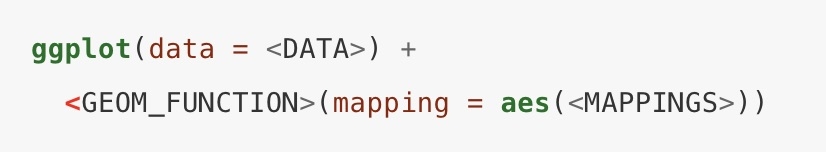
\includegraphics{../données/ggplot_forme_generale.jpg}

\begin{enumerate}
\setcounter{enumi}{2}
\tightlist
\item
  \textbf{aes} pour aestetics indique le nombre de paramètres à passer à
  la fonction \textbf{geom\_function}. Il permet également de spécifier
  des informations sur le graphique.
\end{enumerate}
\end{frame}

\hypertarget{exemples-visualiser-la-distribution-univariuxe9e}{%
\section{Exemples: Visualiser la distribution
univariée}\label{exemples-visualiser-la-distribution-univariuxe9e}}

\begin{frame}[fragile]{Introduction}
\protect\hypertarget{introduction-4}{}
\begin{itemize}
\tightlist
\item
  Nous allons utiliser les données dhs\_ipv
\end{itemize}

\begin{Shaded}
\begin{Highlighting}[]
\FunctionTok{library}\NormalTok{(tidyverse)}

\NormalTok{dhs\_ipv }\OtherTok{\textless{}{-}} \FunctionTok{read\_csv}\NormalTok{(}\StringTok{"../données/dhs\_ipv.csv"}\NormalTok{)}
\NormalTok{dhs\_ipv }\OtherTok{\textless{}{-}}
\NormalTok{  dhs\_ipv }\SpecialCharTok{\%\textgreater{}\%} 
  \FunctionTok{mutate}\NormalTok{(}\AttributeTok{beat\_burnfood\_cat =} \FunctionTok{factor}\NormalTok{(}\FunctionTok{ntile}\NormalTok{(beat\_burnfood, }\DecValTok{4}\NormalTok{), }
                                    \AttributeTok{labels =} \FunctionTok{c}\NormalTok{(}\StringTok{\textquotesingle{}très faible\textquotesingle{}}\NormalTok{, }\StringTok{\textquotesingle{}faible\textquotesingle{}}\NormalTok{, }\StringTok{\textquotesingle{}élevé\textquotesingle{}}\NormalTok{, }\StringTok{\textquotesingle{}très élevé\textquotesingle{}}\NormalTok{)),}
         \AttributeTok{beat\_goesout\_cat =} \FunctionTok{factor}\NormalTok{(}\FunctionTok{ntile}\NormalTok{(beat\_goesout, }\DecValTok{4}\NormalTok{), }
                                   \AttributeTok{labels =} \FunctionTok{c}\NormalTok{(}\StringTok{\textquotesingle{}très faible\textquotesingle{}}\NormalTok{, }\StringTok{\textquotesingle{}faible\textquotesingle{}}\NormalTok{, }\StringTok{\textquotesingle{}élevé\textquotesingle{}}\NormalTok{, }\StringTok{\textquotesingle{}très élevé\textquotesingle{}}\NormalTok{)),}
         \AttributeTok{sec\_school\_cat =} \FunctionTok{factor}\NormalTok{(}\FunctionTok{ntile}\NormalTok{(sec\_school, }\DecValTok{3}\NormalTok{), }
                                 \AttributeTok{labels =} \FunctionTok{c}\NormalTok{(}\StringTok{\textquotesingle{}pauvre\textquotesingle{}}\NormalTok{, }\StringTok{\textquotesingle{}moyen\textquotesingle{}}\NormalTok{, }\StringTok{\textquotesingle{}riche\textquotesingle{}}\NormalTok{)),}
         \AttributeTok{no\_media\_cat =} \FunctionTok{factor}\NormalTok{(}\FunctionTok{ntile}\NormalTok{(no\_media, }\DecValTok{3}\NormalTok{), }
                               \AttributeTok{labels =} \FunctionTok{c}\NormalTok{(}\StringTok{\textquotesingle{}riche\textquotesingle{}}\NormalTok{, }\StringTok{\textquotesingle{}moyen\textquotesingle{}}\NormalTok{, }\StringTok{\textquotesingle{}pauvre\textquotesingle{}}\NormalTok{)))}
\end{Highlighting}
\end{Shaded}
\end{frame}

\begin{frame}[fragile]{Introduction}
\protect\hypertarget{introduction-5}{}
\begin{itemize}
\tightlist
\item
  et les données crsc\_small, que vous connaissez bien.
\end{itemize}

\begin{Shaded}
\begin{Highlighting}[]
\NormalTok{crsc96 }\OtherTok{\textless{}{-}} \FunctionTok{read\_csv}\NormalTok{(}\StringTok{"../données/cora{-}crsc1996{-}E{-}1996\_F1.csv"}\NormalTok{)}
\NormalTok{crsc96\_small }\OtherTok{\textless{}{-}}
\NormalTok{  crsc96 }\SpecialCharTok{\%\textgreater{}\%} 
  \FunctionTok{select}\NormalTok{(sexq, region, age, ageq, q1, q2, q3, q4, q44, q95) }\SpecialCharTok{\%\textgreater{}\%} 
  \FunctionTok{mutate}\NormalTok{(}\AttributeTok{sexe =} \FunctionTok{factor}\NormalTok{(sexq, }\AttributeTok{labels =} \FunctionTok{c}\NormalTok{(}\StringTok{"Homme"}\NormalTok{, }\StringTok{"Femme"}\NormalTok{)),}
         \AttributeTok{q2\_new =} \FunctionTok{factor}\NormalTok{(q2, }
                         \AttributeTok{labels =} \FunctionTok{c}\NormalTok{(}\StringTok{"totally agree"}\NormalTok{, }\StringTok{"agree somewhat"}\NormalTok{, }
                                    \StringTok{"DK/NA"}\NormalTok{, }\StringTok{"disagree somewhat"}\NormalTok{, }\StringTok{"totally disagree"}\NormalTok{)))}
\end{Highlighting}
\end{Shaded}
\end{frame}

\begin{frame}{Distribution univariée}
\protect\hypertarget{distribution-univariuxe9e}{}
\begin{itemize}
\tightlist
\item
  Histogramme : pour variable continue
\item
  Diagramme de barre : pour variable catégorielle
\item
  Diagramme de quartile qui résume cinq indicateurs
\item
  Diagramme circulaire
\end{itemize}
\end{frame}

\begin{frame}[fragile]{Exemple: histogramme}
\protect\hypertarget{exemple-histogramme}{}
\begin{Shaded}
\begin{Highlighting}[]
\FunctionTok{ggplot}\NormalTok{(crsc96\_small) }\SpecialCharTok{+}
  \FunctionTok{geom\_histogram}\NormalTok{(}\FunctionTok{aes}\NormalTok{(}\AttributeTok{x =}\NormalTok{ age))}
\end{Highlighting}
\end{Shaded}

\begin{center}\includegraphics[width=0.7\linewidth]{SICSSM_Seance3.1_Visualisation_files/figure-beamer/unnamed-chunk-5-1} \end{center}
\end{frame}

\begin{frame}{Exemple: histogramme}
\protect\hypertarget{exemple-histogramme-1}{}
\begin{itemize}
\tightlist
\item
  L'histogramme est une méthode courante pour visualiser la distribution
  d'une variable numérique plutôt que d'une variable factorielle.
\item
  Un histogramme divise les données en champs
\item
  L'aire de chaque domaine représente la proportion d'observations qui y
  sont classées.
\item
  La hauteur de chaque case représente la densité, qui est égale à la
  proportion d'observations dans chaque case divisée par la largeur de
  la case.
\item
  Un histogramme se rapproche de la distribution d'une variable.
\end{itemize}
\end{frame}

\begin{frame}{Exemple: histogramme}
\protect\hypertarget{exemple-histogramme-2}{}
\begin{itemize}
\item
  Dans le cadre de cette présentation, je mets des options dans le
  \textbf{chunk} (Vous ne les voyez pas dans la présentation, regarder
  plutôt le fichier .rmd)
\item
  \textbf{out.width} pour préciser la largeur du graphique
\item
  \textbf{message = FALSE} : pour ne pas afficher des messages
\item
  \textbf{warning = FALSE} : pour ne pas afficher des messages
  d'avertissement.
\item
  Il faut les utiliser avec précaution. Les messages et les warning nous
  donnent des informations, par exemple sur les valeurs manquantes.
\end{itemize}
\end{frame}

\begin{frame}[fragile]{Exemple: histogramme}
\protect\hypertarget{exemple-histogramme-3}{}
\begin{itemize}
\tightlist
\item
  Voici ce que vous obtenez si je ne les mets pas.
\end{itemize}

\begin{Shaded}
\begin{Highlighting}[]
\FunctionTok{ggplot}\NormalTok{(dhs\_ipv) }\SpecialCharTok{+}
  \FunctionTok{geom\_histogram}\NormalTok{(}\FunctionTok{aes}\NormalTok{(}\AttributeTok{x =}\NormalTok{ beat\_burnfood))}
\end{Highlighting}
\end{Shaded}

\begin{verbatim}
## `stat_bin()` using `bins = 30`. Pick better value with `binwidth`.
\end{verbatim}

\begin{verbatim}
## Warning: Removed 31 rows containing non-finite values (`stat_bin()`).
\end{verbatim}

\includegraphics{SICSSM_Seance3.1_Visualisation_files/figure-beamer/unnamed-chunk-6-1.pdf}
\end{frame}

\begin{frame}{Exemple: Diagramme en bâtons ou à barres}
\protect\hypertarget{exemple-diagramme-en-buxe2tons-ou-uxe0-barres}{}
\begin{itemize}
\tightlist
\item
  Pour résumer la distribution d'une variable \textbf{facteur} ou d'une
  \textbf{variable factorielle} (ou d'une variable catégorielle ou
  qualitative) avec plusieurs catégories, un simple tableau avec des
  comptes ou des proportions est souvent suffisant.
\item
  Cependant, il est également possible d'utiliser un graphique en barres
  pour visualiser la distribution.
\end{itemize}
\end{frame}

\begin{frame}[fragile]{Exemple: Diagramme en bâtons}
\protect\hypertarget{exemple-diagramme-en-buxe2tons}{}
\begin{Shaded}
\begin{Highlighting}[]
\FunctionTok{ggplot}\NormalTok{(crsc96\_small) }\SpecialCharTok{+}
  \FunctionTok{geom\_bar}\NormalTok{(}\FunctionTok{aes}\NormalTok{(}\AttributeTok{x =}\NormalTok{ q2\_new))}
\end{Highlighting}
\end{Shaded}

\begin{center}\includegraphics[width=0.7\linewidth]{SICSSM_Seance3.1_Visualisation_files/figure-beamer/unnamed-chunk-7-1} \end{center}
\end{frame}

\begin{frame}{Exemple: Diagramme en bâtons}
\protect\hypertarget{exemple-diagramme-en-buxe2tons-1}{}
\begin{itemize}
\tightlist
\item
  Dans les graphiques précédents, l'ordonnée (y) est indiqué en
  effectif. Ceci pose un problème de comparaison entre différents
  échantillons.
\item
  Dans ce cas, il faut plutôt utiliser les proportions.
\end{itemize}
\end{frame}

\begin{frame}[fragile]{Exemple: Diagramme en bâtons}
\protect\hypertarget{exemple-diagramme-en-buxe2tons-2}{}
\begin{Shaded}
\begin{Highlighting}[]
\FunctionTok{ggplot}\NormalTok{(crsc96\_small) }\SpecialCharTok{+}
  \FunctionTok{geom\_bar}\NormalTok{(}\FunctionTok{aes}\NormalTok{(}\AttributeTok{x =}\NormalTok{ q2\_new, }\AttributeTok{y =}\NormalTok{ ..prop.., }\AttributeTok{group =} \DecValTok{1}\NormalTok{))}
\end{Highlighting}
\end{Shaded}

\begin{center}\includegraphics[width=0.7\linewidth]{SICSSM_Seance3.1_Visualisation_files/figure-beamer/unnamed-chunk-8-1} \end{center}
\end{frame}

\begin{frame}{Exemple: Diagramme en bâtons}
\protect\hypertarget{exemple-diagramme-en-buxe2tons-3}{}
\begin{itemize}
\item
  Que se passe-t-il si vous ne mettez pas \textbf{group = 1}
\item
  On peut représenter ce diagramme par un diagramme circulaire. Comment
  créer un diagramme circulaire?
\end{itemize}
\end{frame}

\begin{frame}[fragile]{Diagramme circulaire}
\protect\hypertarget{diagramme-circulaire}{}
\url{https://ggplot2.tidyverse.org/reference/coord_polar.html}

\begin{Shaded}
\begin{Highlighting}[]
\FunctionTok{ggplot}\NormalTok{(crsc96\_small) }\SpecialCharTok{+}
  \FunctionTok{geom\_bar}\NormalTok{(}\FunctionTok{aes}\NormalTok{(}\AttributeTok{x =} \FunctionTok{factor}\NormalTok{(}\DecValTok{1}\NormalTok{), }\AttributeTok{fill =}\NormalTok{ q2\_new), }\AttributeTok{width =} \DecValTok{1}\NormalTok{) }\SpecialCharTok{+} 
  \FunctionTok{coord\_polar}\NormalTok{(}\StringTok{"y"}\NormalTok{, }\AttributeTok{start =} \DecValTok{0}\NormalTok{) }
\end{Highlighting}
\end{Shaded}

\begin{center}\includegraphics[width=0.6\linewidth]{SICSSM_Seance3.1_Visualisation_files/figure-beamer/unnamed-chunk-9-1} \end{center}
\end{frame}

\begin{frame}[fragile]{Exemple: Diagramme de quartile}
\protect\hypertarget{exemple-diagramme-de-quartile}{}
\begin{itemize}
\tightlist
\item
  La boîte à moustache représente un autre moyen de visualiser les
  distributions d'une variable numérique.
\item
  Une boîte à moustache visualise \textbf{la médiane}, \textbf{les
  quartiles} et \textbf{l'écart-interquartile} sous la forme d'un seul
  objet.
\end{itemize}

\begin{Shaded}
\begin{Highlighting}[]
\FunctionTok{ggplot}\NormalTok{(crsc96\_small) }\SpecialCharTok{+} 
  \FunctionTok{geom\_boxplot}\NormalTok{(}\FunctionTok{aes}\NormalTok{(}\AttributeTok{y =}\NormalTok{ age))}
\end{Highlighting}
\end{Shaded}

\begin{center}\includegraphics[width=0.5\linewidth]{SICSSM_Seance3.1_Visualisation_files/figure-beamer/unnamed-chunk-10-1} \end{center}
\end{frame}

\begin{frame}[fragile]{Exemple: Diagramme de quartile ou boîte à
moustaches}
\protect\hypertarget{exemple-diagramme-de-quartile-ou-bouxeete-uxe0-moustaches}{}
\begin{itemize}
\item
  C'est particulièrement utile lorsque vous \textbf{comparez la
  distribution de plusieurs variables} en les plaçant côte à côte.
\item
  \texttt{geom\_boxplot} permet de représenter des boîtes à moustaches.
  On lui passe en \textbf{y} (axe des ordonnées) la variable dont on
  veut étudier la répartition (variable quantitative), et en \textbf{x}
  (axe des abscisses) la variable contenant les classes qu'on souhaite
  comparer (variable qualitative).
\end{itemize}
\end{frame}

\hypertarget{exemples-visualiser-la-distribution-bivariuxe9e}{%
\section{Exemples: Visualiser la distribution
bivariée}\label{exemples-visualiser-la-distribution-bivariuxe9e}}

\begin{frame}[fragile]{Croisement de deux variables qualitatives}
\protect\hypertarget{croisement-de-deux-variables-qualitatives}{}
\begin{Shaded}
\begin{Highlighting}[]
\FunctionTok{ggplot}\NormalTok{(crsc96\_small) }\SpecialCharTok{+}
  \FunctionTok{geom\_bar}\NormalTok{(}\FunctionTok{aes}\NormalTok{(}\AttributeTok{x =}\NormalTok{ sexe, }\AttributeTok{fill =}\NormalTok{ q2\_new))}
\end{Highlighting}
\end{Shaded}

\begin{center}\includegraphics[width=0.7\linewidth]{SICSSM_Seance3.1_Visualisation_files/figure-beamer/unnamed-chunk-11-1} \end{center}

\begin{itemize}
\tightlist
\item
  Ce graphique nous donne pour chaque sexe, le nombre de personnes qui
  sont dans chaque catégorie de la variable dépendante.
\item
  Il a cependant un problème, c'est difficile de comparer les nombres
  bruts. Il faut des pourcentages.
\end{itemize}
\end{frame}

\begin{frame}[fragile]{Croisement de deux variables qualitatives}
\protect\hypertarget{croisement-de-deux-variables-qualitatives-1}{}
\begin{Shaded}
\begin{Highlighting}[]
\FunctionTok{ggplot}\NormalTok{(crsc96\_small) }\SpecialCharTok{+}
  \FunctionTok{geom\_bar}\NormalTok{(}\FunctionTok{aes}\NormalTok{(}\AttributeTok{x =}\NormalTok{ sexe, }\AttributeTok{fill =}\NormalTok{ q2\_new), }\AttributeTok{position =} \StringTok{"fill"}\NormalTok{)  }
\end{Highlighting}
\end{Shaded}

\begin{center}\includegraphics[width=0.6\linewidth]{SICSSM_Seance3.1_Visualisation_files/figure-beamer/unnamed-chunk-12-1} \end{center}

\begin{itemize}
\tightlist
\item
  On voit clairement la différence d'opinion entres les hommes et les
  femmes.
\end{itemize}
\end{frame}

\begin{frame}[fragile]{Croisement de deux variables qualitatives}
\protect\hypertarget{croisement-de-deux-variables-qualitatives-2}{}
\begin{itemize}
\tightlist
\item
  On peut changer les couleurs, on verra cela plus loin.
\item
  \url{http://www.sthda.com/french/wiki/couleurs-dans-r}
\end{itemize}

\begin{Shaded}
\begin{Highlighting}[]
\FunctionTok{ggplot}\NormalTok{(crsc96\_small) }\SpecialCharTok{+}
  \FunctionTok{geom\_bar}\NormalTok{(}\FunctionTok{aes}\NormalTok{(}\AttributeTok{x =}\NormalTok{ sexe, }\AttributeTok{fill =}\NormalTok{ q2\_new), }\AttributeTok{position =} \StringTok{"fill"}\NormalTok{) }\SpecialCharTok{+}
  \FunctionTok{scale\_fill\_brewer}\NormalTok{(}\AttributeTok{palette=}\StringTok{"PRGn"}\NormalTok{) }
\end{Highlighting}
\end{Shaded}

\begin{center}\includegraphics[width=0.6\linewidth]{SICSSM_Seance3.1_Visualisation_files/figure-beamer/unnamed-chunk-13-1} \end{center}

\begin{Shaded}
\begin{Highlighting}[]
\CommentTok{\# Changer PRGn avec un chiffre}
\end{Highlighting}
\end{Shaded}
\end{frame}

\begin{frame}{Croisement d'une variable quantitative et d'une variable
qualitative}
\protect\hypertarget{croisement-dune-variable-quantitative-et-dune-variable-qualitative}{}
\begin{itemize}
\tightlist
\item
  Croiser une variable quantitative et une variable qualitative, c'est
  essayer de voir si les valeurs de la variable quantitative se
  répartissent différemment selon les catégories d'appartenance de la
  variable qualitative.
\end{itemize}
\end{frame}

\begin{frame}[fragile]{Croisement d'une variable quantitative et d'une
variable qualitative}
\protect\hypertarget{croisement-dune-variable-quantitative-et-dune-variable-qualitative-1}{}
\begin{itemize}
\tightlist
\item
  Avant de présenter ce diagramme, regardons un peu la distribution de
  la variable beat\_burnfood par région.
\end{itemize}

\begin{Shaded}
\begin{Highlighting}[]
\NormalTok{a }\OtherTok{\textless{}{-}}
\FunctionTok{ggplot}\NormalTok{(dhs\_ipv) }\SpecialCharTok{+} 
  \FunctionTok{geom\_text}\NormalTok{(}\FunctionTok{aes}\NormalTok{(}\AttributeTok{x =}\NormalTok{ region, }\AttributeTok{y =}\NormalTok{ beat\_burnfood, }
                \AttributeTok{label =}\NormalTok{ country, }\AttributeTok{color =}\NormalTok{ region), }\AttributeTok{size =} \DecValTok{2}\NormalTok{)}
\end{Highlighting}
\end{Shaded}
\end{frame}

\begin{frame}[fragile]{Croisement d'une variable quantitative et d'une
variable qualitative}
\protect\hypertarget{croisement-dune-variable-quantitative-et-dune-variable-qualitative-2}{}
\begin{Shaded}
\begin{Highlighting}[]
\NormalTok{a }
\end{Highlighting}
\end{Shaded}

\begin{center}\includegraphics[width=0.7\linewidth]{SICSSM_Seance3.1_Visualisation_files/figure-beamer/unnamed-chunk-15-1} \end{center}

\begin{itemize}
\tightlist
\item
  Commenter ce graphique.
\end{itemize}
\end{frame}

\begin{frame}[fragile]{Croisement d'une variable quantitative et d'une
variable qualitative}
\protect\hypertarget{croisement-dune-variable-quantitative-et-dune-variable-qualitative-3}{}
\begin{Shaded}
\begin{Highlighting}[]
\NormalTok{a }\SpecialCharTok{+} 
  \FunctionTok{theme}\NormalTok{(}\AttributeTok{axis.text.x =} \FunctionTok{element\_text}\NormalTok{(}\AttributeTok{angle =} \DecValTok{20}\NormalTok{, }\AttributeTok{hjust =} \DecValTok{1}\NormalTok{),}
        \AttributeTok{legend.position =} \StringTok{"none"}\NormalTok{)}
\end{Highlighting}
\end{Shaded}

\begin{center}\includegraphics[width=0.6\linewidth]{SICSSM_Seance3.1_Visualisation_files/figure-beamer/unnamed-chunk-16-1} \end{center}
\end{frame}

\begin{frame}[fragile]{Exemple: Diagramme de quartile}
\protect\hypertarget{exemple-diagramme-de-quartile-1}{}
\begin{itemize}
\tightlist
\item
  Le diagramme de quartile permet de synthétiser l'information contenue
  dans ce nuage de points pour une comparaison plus efficiente.
\end{itemize}

\begin{Shaded}
\begin{Highlighting}[]
\NormalTok{b }\OtherTok{\textless{}{-}} \FunctionTok{ggplot}\NormalTok{(dhs\_ipv) }\SpecialCharTok{+} 
  \FunctionTok{geom\_boxplot}\NormalTok{(}\FunctionTok{aes}\NormalTok{(}\AttributeTok{x =}\NormalTok{ region, }\AttributeTok{y =}\NormalTok{ beat\_burnfood))}
\NormalTok{b}
\end{Highlighting}
\end{Shaded}

\begin{center}\includegraphics[width=0.6\linewidth]{SICSSM_Seance3.1_Visualisation_files/figure-beamer/unnamed-chunk-17-1} \end{center}

\begin{itemize}
\tightlist
\item
  Note : x doit être une variable qualitative, et y une variable
  quantitative.
\end{itemize}
\end{frame}

\begin{frame}[fragile]{Exemple: Diagramme de quartile}
\protect\hypertarget{exemple-diagramme-de-quartile-2}{}
\begin{Shaded}
\begin{Highlighting}[]
\NormalTok{c }\OtherTok{\textless{}{-}} \FunctionTok{ggplot}\NormalTok{(dhs\_ipv) }\SpecialCharTok{+} 
  \FunctionTok{geom\_boxplot}\NormalTok{(}\FunctionTok{aes}\NormalTok{(}\AttributeTok{x =}\NormalTok{ region, }\AttributeTok{y =}\NormalTok{ sec\_school))}
\NormalTok{c}
\end{Highlighting}
\end{Shaded}

\begin{center}\includegraphics[width=0.6\linewidth]{SICSSM_Seance3.1_Visualisation_files/figure-beamer/unnamed-chunk-18-1} \end{center}
\end{frame}

\begin{frame}{Exemple: Diagramme de quartile}
\protect\hypertarget{exemple-diagramme-de-quartile-3}{}
\begin{itemize}
\tightlist
\item
  Commencez-vous par tirer une petite conclusion ici?
\item
  Pour bien visualiser le tout, il faut les mettre dans un même
  graphique. La commande \textbf{ggarrange} du package \textbf{ggpubr}
  vous permet de faire cela.
\end{itemize}
\end{frame}

\begin{frame}[fragile]{Exemple: Diagramme de quartile}
\protect\hypertarget{exemple-diagramme-de-quartile-4}{}
\begin{Shaded}
\begin{Highlighting}[]
\CommentTok{\#install.packages("ggpubr")}
\FunctionTok{library}\NormalTok{(ggpubr)}
\FunctionTok{ggarrange}\NormalTok{(b, c, }\AttributeTok{ncol =} \DecValTok{2}\NormalTok{)}
\end{Highlighting}
\end{Shaded}

\begin{center}\includegraphics[width=0.7\linewidth]{SICSSM_Seance3.1_Visualisation_files/figure-beamer/unnamed-chunk-19-1} \end{center}
\end{frame}

\hypertarget{association-entre-deux-variables-quantitatives}{%
\section{Association entre deux variables
quantitatives}\label{association-entre-deux-variables-quantitatives}}

\begin{frame}[fragile]{Corrélation linéaire : Croisement de deux
variables quantitatives}
\protect\hypertarget{corruxe9lation-linuxe9aire-croisement-de-deux-variables-quantitatives}{}
\begin{Shaded}
\begin{Highlighting}[]
\FunctionTok{ggplot}\NormalTok{(dhs\_ipv) }\SpecialCharTok{+}
  \FunctionTok{geom\_point}\NormalTok{(}\FunctionTok{aes}\NormalTok{(}\AttributeTok{x =}\NormalTok{ sec\_school, }\AttributeTok{y =}\NormalTok{ beat\_burnfood)) }
\end{Highlighting}
\end{Shaded}

\begin{center}\includegraphics[width=0.65\linewidth]{SICSSM_Seance3.1_Visualisation_files/figure-beamer/unnamed-chunk-20-1} \end{center}
\end{frame}

\begin{frame}[fragile]{Corrélation linéaire : Croisement de deux
variables quantitatives}
\protect\hypertarget{corruxe9lation-linuxe9aire-croisement-de-deux-variables-quantitatives-1}{}
\begin{Shaded}
\begin{Highlighting}[]
\FunctionTok{ggplot}\NormalTok{(dhs\_ipv) }\SpecialCharTok{+}
  \FunctionTok{geom\_point}\NormalTok{(}\FunctionTok{aes}\NormalTok{(}\AttributeTok{x =}\NormalTok{ no\_media, }\AttributeTok{y =}\NormalTok{ beat\_burnfood)) }
\end{Highlighting}
\end{Shaded}

\begin{center}\includegraphics[width=0.7\linewidth]{SICSSM_Seance3.1_Visualisation_files/figure-beamer/unnamed-chunk-21-1} \end{center}
\end{frame}

\hypertarget{remarques}{%
\section{Remarques}\label{remarques}}

\begin{frame}{Remarques}
\protect\hypertarget{remarques-1}{}
\begin{itemize}
\tightlist
\item
  Les annotations graphiques sont très utiles pour mettre en évidence
  les messages clés.
\item
  Dans un bulletin ou un rapport statistique, tous les graphiques
  doivent être étiquetés comme des figures et numérotés, en fonction de
  leur ordre d'apparition.
\item
  Ecrire clairement les titres : préciser la région et la période.
\item
  Soyez concis, en nommant les principaux axes du graphique.
\item
  Le texte du graphique doit être horizontal.
\item
  Si les étiquettes ne tiennent pas dans l'espace requis, transposez le
  graphique ou convertissez les unités.

  \begin{itemize}
  \tightlist
  \item
    Elles doivent être concises et pertinentes.
  \item
    Placez les sur le graphique aussi près que possible des points de
    données qui vous intéressent.
  \end{itemize}
\item
  Indiquer la source
\end{itemize}
\end{frame}

\begin{frame}{Remarques}
\protect\hypertarget{remarques-2}{}
\url{https://slideplayer.fr/slide/10114066/}
\end{frame}

\begin{frame}{Pour aller plus loin}
\protect\hypertarget{pour-aller-plus-loin}{}
\begin{itemize}[<+->]
\tightlist
\item
  Plus dans aes : \textbf{mappage} : c'est une mise en relation entre un
  \textbf{attribut graphique du geom} et une variable du tableau de
  données.
\item
  Changer les couleurs (\emph{color}), la taille (\emph{size}), la
  position (\emph{position}), la transparence (\emph{alpha}), le
  remplissage (\emph{fill})
\end{itemize}

\begin{itemize}[<+->]
\tightlist
\item
  \textbf{Facets} : le \textbf{faceting} permet d'effectuer plusieurs
  fois le même graphique selon les valeurs d'une ou plusieurs variables
  qualitatives (notre \emph{group\_by}): facet\_wrap, facet\_grid
\end{itemize}

\begin{itemize}[<+->]
\tightlist
\item
  Les \textbf{scales} : ils permettent de modifier la manière dont un
  attribut graphique va être relié aux valeurs d'une variable, et dont
  la légende correspondante va être affichée.
\end{itemize}

\begin{itemize}[<+->]
\tightlist
\item
  Les \textbf{thèmes} : ils permettent de contrôler l'affichage de tous
  les éléments du graphique qui ne sont pas reliés aux données :
  \textbf{titres}, \textbf{grilles}, \textbf{fonds}, etc.
  \url{https://ggplot2.tidyverse.org/reference/theme.html}
\end{itemize}
\end{frame}

\begin{frame}[fragile]{Pour aller plus loin : exemple 1}
\protect\hypertarget{pour-aller-plus-loin-exemple-1}{}
\begin{Shaded}
\begin{Highlighting}[]
\NormalTok{d }\OtherTok{\textless{}{-}} \FunctionTok{ggplot}\NormalTok{(dhs\_ipv) }\SpecialCharTok{+}
  \FunctionTok{geom\_point}\NormalTok{(}\FunctionTok{aes}\NormalTok{(}\AttributeTok{x =}\NormalTok{ no\_media, }\AttributeTok{y =}\NormalTok{ beat\_burnfood, }
                 \AttributeTok{color =}\NormalTok{ region)) }\SpecialCharTok{+}
  \FunctionTok{geom\_smooth}\NormalTok{(}\FunctionTok{aes}\NormalTok{(}\AttributeTok{x =}\NormalTok{ no\_media, }\AttributeTok{y =}\NormalTok{ beat\_burnfood, }
                  \AttributeTok{color =}\NormalTok{ region), }
              \AttributeTok{method =}\NormalTok{ lm, }\AttributeTok{se =} \ConstantTok{FALSE}\NormalTok{,  }\AttributeTok{formula =}\NormalTok{ y }\SpecialCharTok{\textasciitilde{}}\NormalTok{ x) }\SpecialCharTok{+} 
  \FunctionTok{labs}\NormalTok{(}\AttributeTok{title =} \StringTok{"Association entre accès aux médias et attitudes face à la violence"}\NormalTok{,}
       \AttributeTok{x =} \StringTok{"Non accès aux médias (\%)"}\NormalTok{,}
       \AttributeTok{y =} \StringTok{"Battre si brûle la nourriture (\%)"}\NormalTok{) }\SpecialCharTok{+}
  \FunctionTok{theme}\NormalTok{(}\AttributeTok{legend.position =} \StringTok{"bottom"}\NormalTok{, }\AttributeTok{legend.direction =} \StringTok{"horizontal"}\NormalTok{)}
\end{Highlighting}
\end{Shaded}
\end{frame}

\begin{frame}[fragile]{Pour aller plus loin : exemple 1}
\protect\hypertarget{pour-aller-plus-loin-exemple-1-1}{}
\begin{Shaded}
\begin{Highlighting}[]
\NormalTok{d}
\end{Highlighting}
\end{Shaded}

\begin{center}\includegraphics[width=0.7\linewidth]{SICSSM_Seance3.1_Visualisation_files/figure-beamer/unnamed-chunk-23-1} \end{center}
\end{frame}

\begin{frame}[fragile]{Pour aller plus loin : exemple 2}
\protect\hypertarget{pour-aller-plus-loin-exemple-2}{}
\begin{Shaded}
\begin{Highlighting}[]
\NormalTok{e }\OtherTok{\textless{}{-}} \FunctionTok{ggplot}\NormalTok{(dhs\_ipv) }\SpecialCharTok{+}
  \FunctionTok{geom\_point}\NormalTok{(}\FunctionTok{aes}\NormalTok{(}\AttributeTok{x =}\NormalTok{ no\_media, }\AttributeTok{y =}\NormalTok{ beat\_burnfood, }\AttributeTok{color =}\NormalTok{ beat\_burnfood)) }\SpecialCharTok{+}
  \FunctionTok{scale\_color\_gradient}\NormalTok{(}\StringTok{"beat\_burnfood"}\NormalTok{, }\AttributeTok{low =} \StringTok{"blue"}\NormalTok{, }\AttributeTok{high =} \StringTok{"red"}\NormalTok{) }\SpecialCharTok{+}
\CommentTok{\# scale\_size(range = c(0,4), breaks = c(15, 25, 35, 45)) +}
  \FunctionTok{facet\_wrap}\NormalTok{(}\SpecialCharTok{\textasciitilde{}}\NormalTok{region) }\SpecialCharTok{+}
  \FunctionTok{labs}\NormalTok{(}\AttributeTok{title =} \StringTok{"Association entre accès aux médias et attitudes face à la violence"}\NormalTok{,}
       \AttributeTok{x =} \StringTok{"Non accès aux médias (\%)"}\NormalTok{,}
       \AttributeTok{y =} \StringTok{"Battre si brûle la nourriture (\%)"}\NormalTok{,}
       \StringTok{"region"} \OtherTok{=} \StringTok{"Région"}\NormalTok{)  }\SpecialCharTok{+}
  \FunctionTok{theme\_bw}\NormalTok{() }
\end{Highlighting}
\end{Shaded}
\end{frame}

\begin{frame}[fragile]{Pour aller plus loin : exemple 2}
\protect\hypertarget{pour-aller-plus-loin-exemple-2-1}{}
\begin{Shaded}
\begin{Highlighting}[]
\NormalTok{e}
\end{Highlighting}
\end{Shaded}

\begin{center}\includegraphics[width=0.75\linewidth]{SICSSM_Seance3.1_Visualisation_files/figure-beamer/unnamed-chunk-25-1} \end{center}
\end{frame}

\hypertarget{ressources}{%
\section{Ressources}\label{ressources}}

\begin{frame}{Ressources}
\protect\hypertarget{ressources-1}{}
\begin{itemize}
\item
  \url{https://www.google.com/search?q=ggplot+theme\%2C+dont+show+legend\&oq=ggplot+theme\%2C+dont+show+legend\&aqs=chrome}..69i57j0.7717j0j4\&sourceid=chrome\&ie=UTF-8
\item
  \url{https://juba.github.io/tidyverse/08-ggplot2.html\#}

  \begin{itemize}
  \tightlist
  \item
    Fortement recommandé
  \end{itemize}
\item
  \url{https://www.rstudio.com/resources/cheatsheets/}
\item
  \url{http://r4ds.had.co.nz/data-visualisation.html\#aesthetic-mappings}
\item
  \url{http://r-statistics.co/Top50-Ggplot2-Visualizations-MasterList-R-Code.html}
\item
  \url{http://www.cookbook-r.com/Graphs/}
\item
  \url{http://www.ggplot2-exts.org/gallery/}

  \begin{itemize}
  \tightlist
  \item
    Si vous y trouver de la passion\ldots{}
  \end{itemize}
\end{itemize}
\end{frame}

\end{document}
